\section{Implementation}
\label{sec:implementation}

In this section, we describe \libname{}, a library that implements both \ssmr\ and \dssmr{}, and \appname{}, a scalable social network application built with \libname{}. \libname\ and \appname\ were both implemented in Java.

\begin{figure*}
\begin{minipage}[b]{1\linewidth} % A minipage that covers the whole width of the page
\centering
      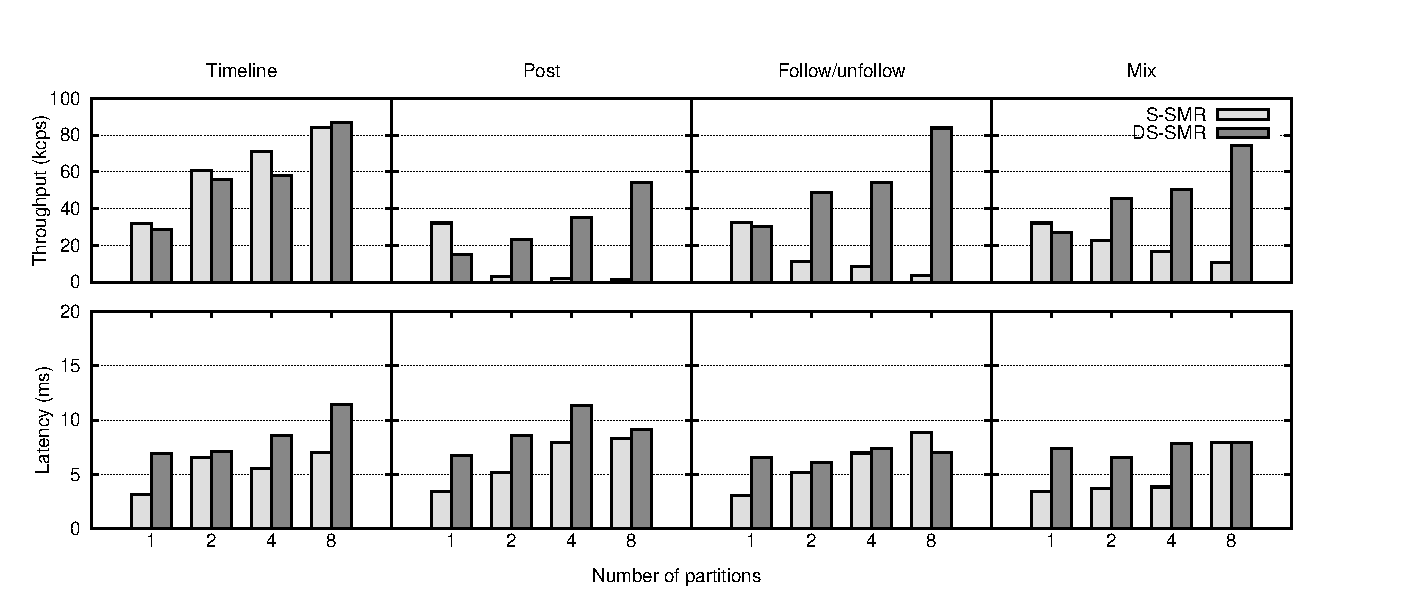
\includegraphics[width=1.0\linewidth]{figures/graphs/strong-locality}
\end{minipage}
\caption{Results of \appname\ running with \ssmr\ and \dssmr{}, for strong-locality workloads. Throughput is show in thousands of commands per second (kcps).}
\label{fig:strongloc}
\end{figure*}

\subsection{\libname}

To implement a replicated service with \libname{}, the developer (i.e., service designer) must extend three classes: PRObject, StateMachine, OracleStateMachine.

\textbf{The PRObject class.} \libname{} supports partial replication (i.e., some objects may be replicated in some partitions, not all). Therefore, when executing a command, a replica might not have local access to some of the objects involved in the execution of the command. The developer informs to \libname{} which object classes are partially replicated by extending the PRObject class. Each object of such class is stored either locally or remotely, but the application code is agnostic to that. All calls to methods of such objects are intercepted by \appname{}, transparently to the developer.

% are you still using the aspect? do methods actually get intercepted by D-Eyrie?

\textbf{The StateMachine class.} This class implements the logic of the server proxy. The application server class must extend the StateMachine class. To execute commands, the developer must provide an implementation for the method executeCommand(Command). The code for such a method is agnostic to the existence of partitions. In other words, it can be exactly the same as the code used to execute commands with classical state-machine replication (i.e., full replication). \libname{} is responsible for handling all communication between partitions and oracle transparently. To start the server, method runStateMachine() is called. Method createObject() also needs to be implemented, where the the developer defines how new state objects are loaded or created.

\textbf{The OracleStateMachine class.} This class implements the logic of the oracle proxy. It extends StateMachine, so the oracle can be deployed similarly to a fault-tolerant partition in the original \ssmr{}. Class OracleStateMachine has a default implementation, but the developer is encouraged to override its methods. Method extractObject(Command) returns the set of objects accessed by the command. It should be overriden by the application so that the client proxy can relocate all necessary objects to a destination partition before executing the application command.
% didn't understand this: "in the case there are hidden objects in the command."
Method getTargetPartition(Set$\langle$Object$\rangle$) returns a particular partition to which objects should be moved, when they are not in the same partition yet, in order to execute an application command that accesses those objects. The default implementation of the method returns a random partition. The developer can override it in order to further improve the distribution of objects among partitions.
For instance, the destination partition could be chosen based on an attribute of the objects passed to the method.

The client proxy is implemented in class Client, which handles all communication of the application client with the partitioned service. The client proxy provides methods sendCreate(Command, CallbackHandler), sendAccess(Command, CallbackHandler), and sendDelete(Command, CallbackHandler). The client proxy's default behavior is to keep retrying commands (and fallback to \dssmr\ in case of too many retries) and only call back the application client when the command has been successfully executed.
However, the developer can change this behavior by overriding the error() method of CallbackHandler. The error() method is called when a $retry$ reply is received.

% i don't understand what the application can actually change with the error() method

\subsection{\appname}

We implemented \appname{}, a social network application similar to Twitter, using \libname{}. Twitter is an online social networking service in which users can post 140-character messages and read posted messages of other users. The API consists basically of: post (user publishes a message), follow (user starts following another user), unfollow(user stops following someone), and getTimeline (user requests messages of all people whom the user follows).

State partitioning in \appname\ is based on users' interest. A function $f(uid)$ returns the partition that user with id $uid$ should belong to, based on the user's interest. Function $f$ is implemented in method getObjectPlacement(User) of class \appname{}Oracle, which extends OracleStateMachine (class User extends PRObject). Taking into account that a typical user probably spends more time reading messages (i.e., issuing getTimeline) than writing them (i.e., issuing post), we decided to optimize getTimeline to be single-partition. This means that, when a user requests his or her timeline, all messages should be available in the partition that stores that user’s data, in the form of a materialized timeline (similarly to a materialized view in a database). To make this possible, whenever a post request is executed, the message is inserted into the materialized timeline of all users that follow the one that is posting. Also, when a user starts following another user, the messages of the followed user are inserted into the follower’s materialized timeline as part of the command execution; likewise, they are removed when a user stops following another user. Because of this design decision, every getTimeline request accesses only one partition, follow and unfollow requests access to objects reside on most two partitions, and post requests access up to object on all partitions. The \appname{} client does not need any knowledge about partitions, since it uses method sendAccessCommand(command) of the \dssmr{} client proxy to issue its commands.

One detail about the post request is that it needs access to all users that follow the user issuing the post.
%Thus the list of follower need to be attached in the post command. However, the (Chirper) client cannot know for sure who follows the user: it keeps a cache of followers, but such cache can become stale if a different user starts following the poster.
To ensure linearizability when executing a post request, the \appname\ server overrides the extractObject(command) method to check if all followers that will be accessed by the command are available in the local partition (i.e., the partition of the server executing the post command).
If this is the case, the request is executed.
Otherwise, the server sends a $retry(\gamma)$ message, where $\gamma$ is the complete set of followers of the user who was posting.
Then, the \appname\ server proceeds to the next command.
Upon receiving the $retry(\gamma)$ message, the client proxy tries to move all users in $\gamma$ to the same partition before retrying to execute the post command.
